% !Mode:: "TeX:UTF-8"
% !TEX program  = xelatex
\section{Methods}
\subsection{Autoencoder}
The autoencoder is composed of an encoder network and a decoder network \cite{wang2016auto}. The encoder network aims to model the distribution of the data points $P(x)$ in a high dimensional space $X$ and represents them by low dimensional latent variables $z$. Then, the decoder network maps the low-dimensionality variables $z$ back to the original high dimensional space $X$. To ensure that the generated latent representation $z$ can extract the intrinsic features of the data points, autoencoder tries to keep the reconstructed outputs and the original inputs as close as possible. The structure of an autoencoder are shown in Figure \ref{modelae}

\begin{figure}[htb!]
    \centering
    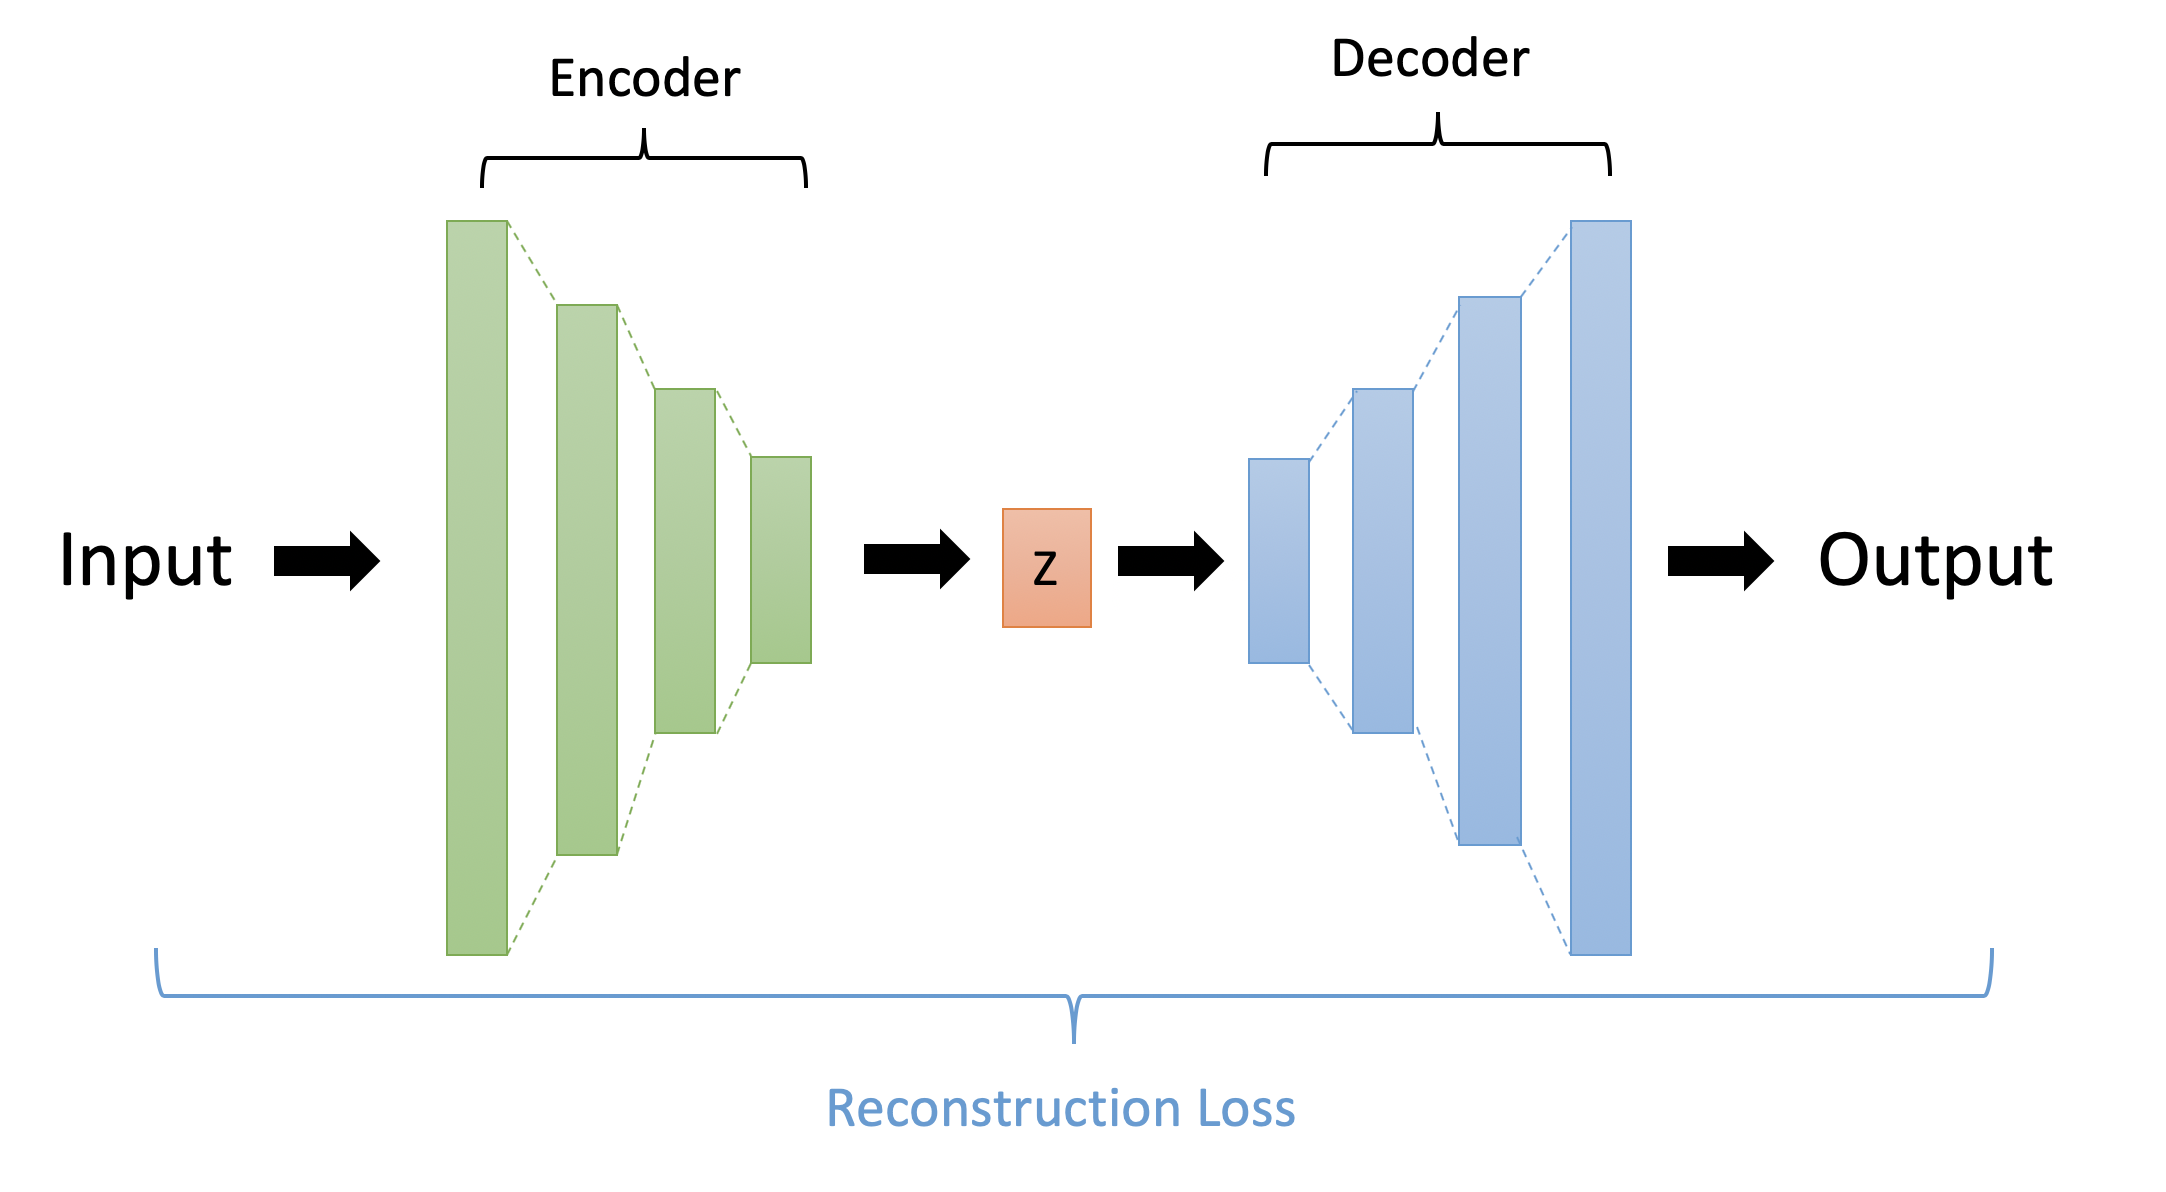
\includegraphics[width=1\textwidth]{figures/myfigures/ae.png}
    \caption{The structure of autoencoder}
    \label{modelae}
\end{figure}

\subsection{Variational autoencoder}
However, the autoencoder only minimize the reconstruction error between the input data and the decoded data. The network is likely to be overfitted, which may cause bad effects to the visualization of data points. So, the variational autoencoder model adds regularizations to the original autoencoder in order to avoid overfitting and get more meaningful visualization results. Instead of encoding the data as a point in the latent space, VAE encodes the data as a distribution in the latent space. A point is sampled from that distribution each time to feed into the decoder network. The structure of an autoencoder are shown in Figure \ref{modelvae}

\begin{figure}[htb!]
    \centering
    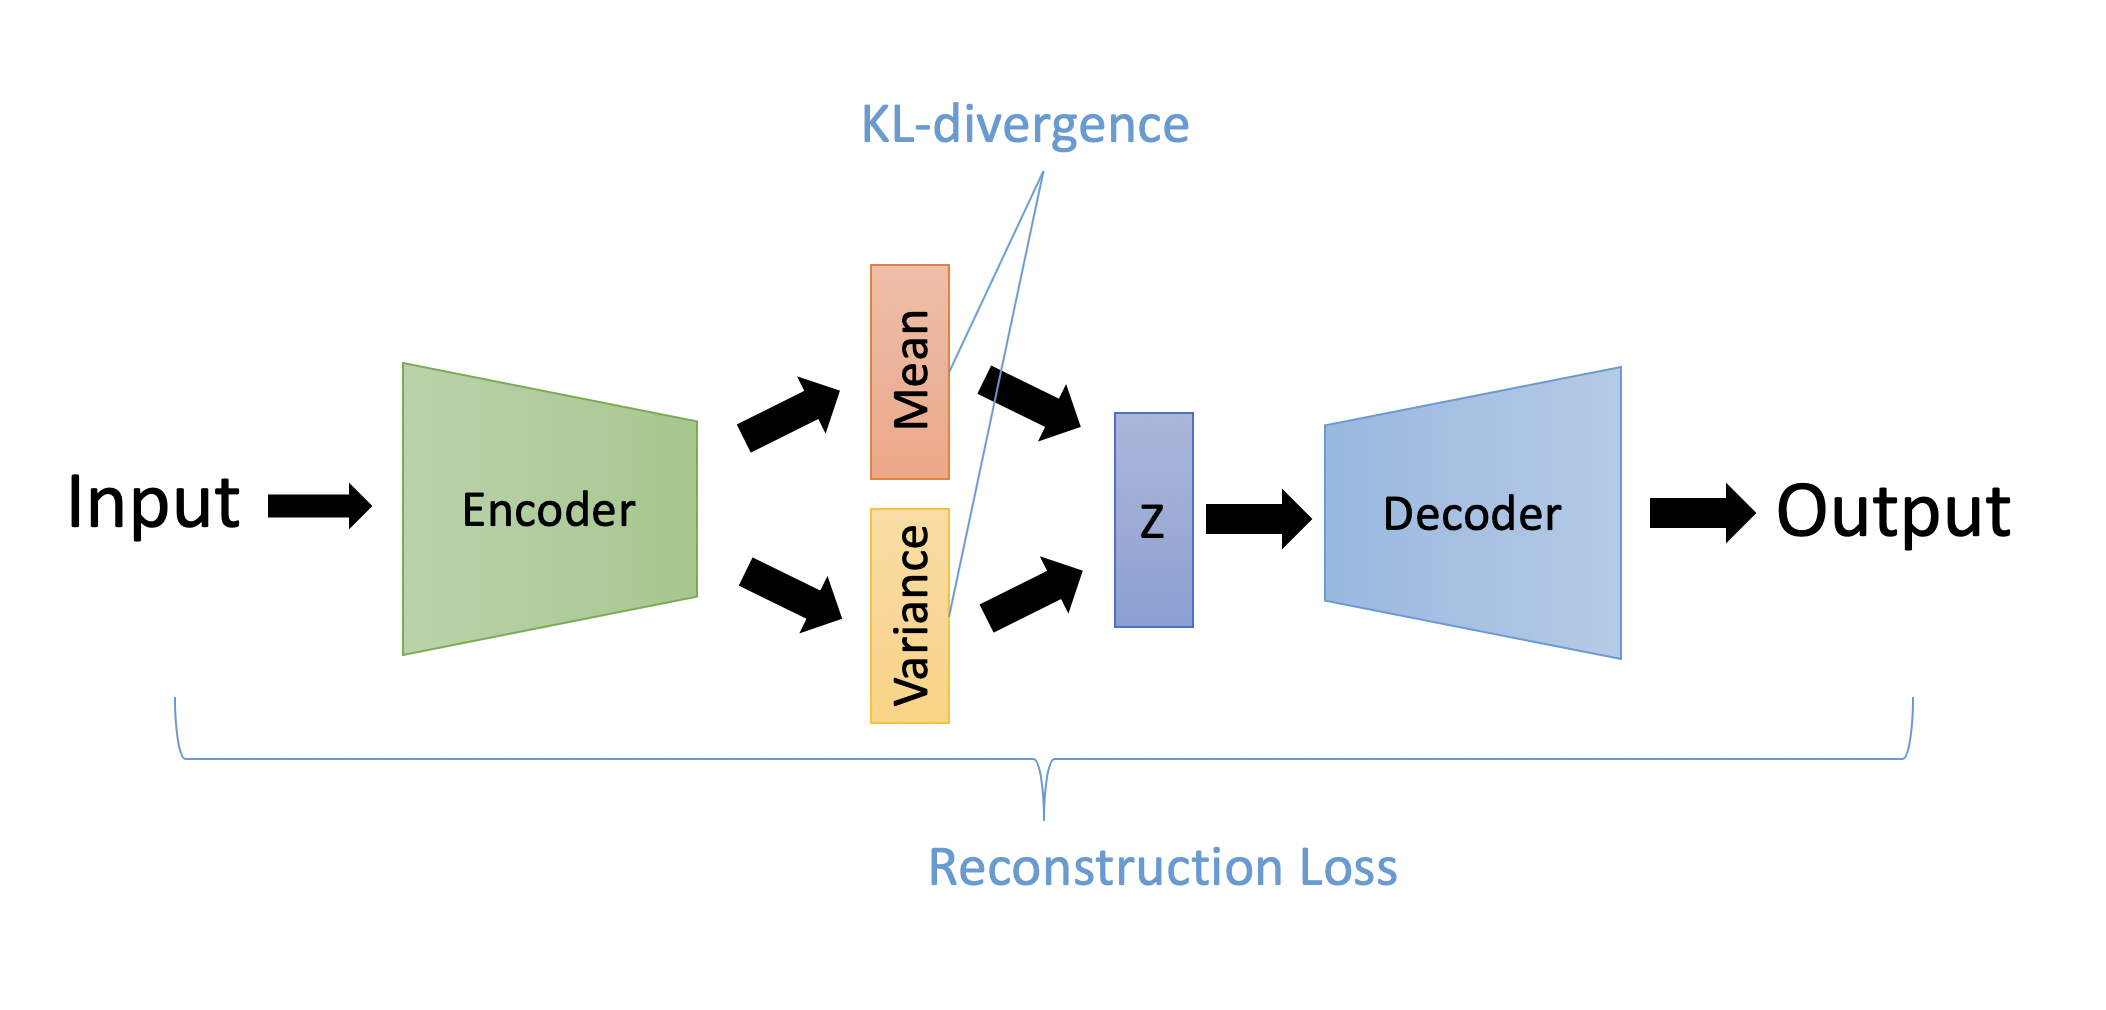
\includegraphics[width=1\textwidth]{figures/myfigures/vae.png}
    \caption{The structure of variational autoencoder}
    \label{modelvae}
\end{figure}

Theoretically, the optimal distribution of $z$ follows the posterior probability $P(z|x)$, which is usually intractable. Therefore, VAE hopes to use a variational probability $Q(z|x)$ to approximate that posterior probability \cite{doersch2016tutorial}. It minimizes the $KL$-divergence between them:
\begin{equation}
\boldsymbol{D}[\boldsymbol{Q}(\boldsymbol{z} | \boldsymbol{X}) \| \boldsymbol{P}(\boldsymbol{z} | \boldsymbol{X})]=\mathbf{E}_{z \sim Q}[\log \boldsymbol{Q}(\boldsymbol{z} | \boldsymbol{X})-\log \boldsymbol{P}(\boldsymbol{z} | \boldsymbol{X})]
\end{equation}
Using Bayes rule and reordering the formula, it is equivalent to maximizing the following equation:
\begin{equation}
\mathbf{E}_{z \sim Q}[\log \boldsymbol{P}(\boldsymbol{X} | \boldsymbol{z})]-\boldsymbol{D}[\boldsymbol{Q}(\boldsymbol{z} | \boldsymbol{X}) \| \boldsymbol{P}(\boldsymbol{z})]
\end{equation}
Where $E$ means the expectation of $z$ which is sampled from distribution $Q$. $P(X|z)$ can be modeled by a decoder and $Q(z|X)$ can be modeled by an encoder. The first term can be viewed as the reconstruction loss. The second term minimizes the $KL$-divergence between the latent variable distribution and the normal distribution. It forces the latent variables follow the standard Gaussian distribution.

\subsection{Model structure}
I used a modified variational autoencoder \cite{Kingma2014} to reduce the dimensionality of the single cell RNA-seq data. The whole structure of ZIVA is shown in figure \ref{modelstru}. The details of model design and optimization algorithms are described as following. 
\begin{figure}[htb!]
    \centering
    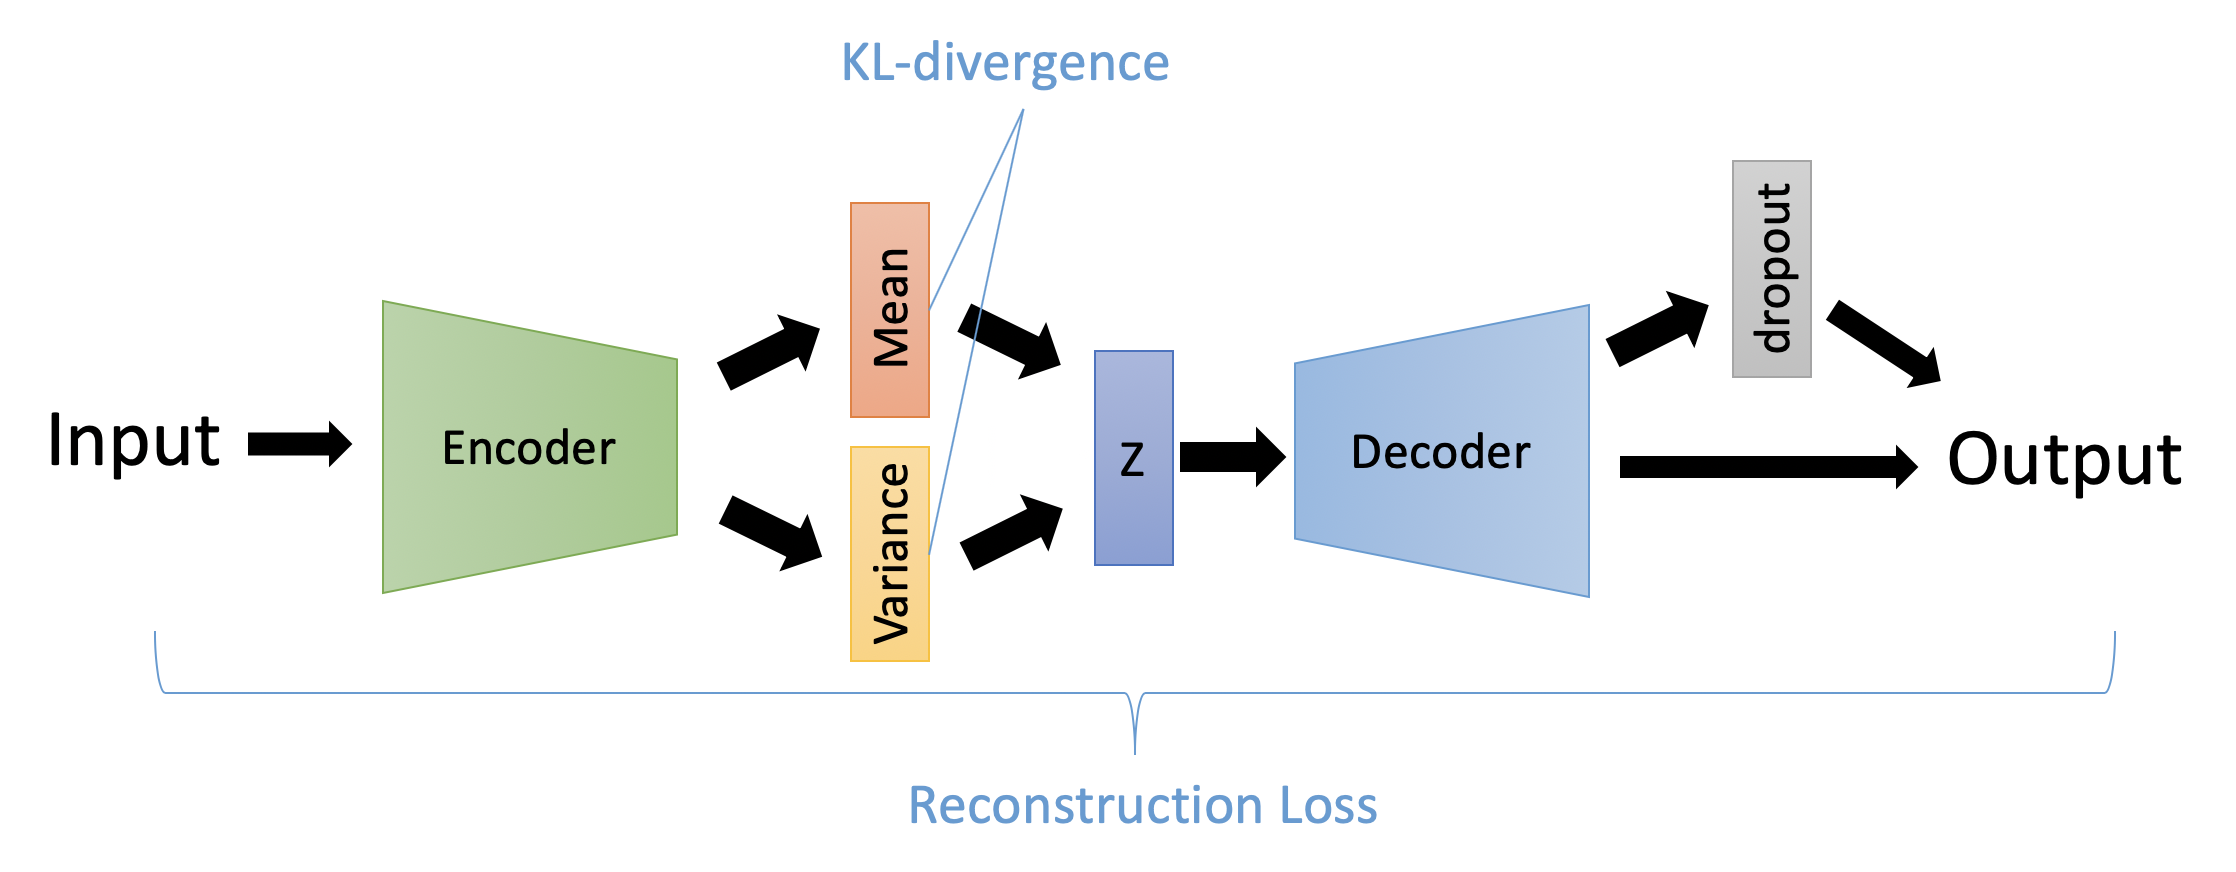
\includegraphics[width=1\textwidth]{figures/myfigures/ZIVA.png}
    \caption{The whole structure of ZIVA}
    \label{modelstru}
\end{figure}

\vspace{0.5cm}
\noindent\emph{Input layer} \\ The ZIVA model uses the expression value matrix from single cell RNA sequencing data as inputs. Then, the data were performed log transformation to improve robustness of the model.  Also, the expression of genes in a cell were re-scaled to 0-1 by dividing the maximum gene expression value in the same cell. 

\vspace{0.5cm}
\noindent\emph{Dropout layer} \\ A dropout layer \cite{baldi2013understanding} is followed by the input layer. This layer sets some value to zero to get better performance of learning \cite{vincent2008extracting}. It can be viewed as some artificial dropouts which can force the model to learn to aid the bad effect of dropout noises. 

\vspace{0.5cm}
\noindent\emph{Encoder network} \\
The encoder network aims to represent the data points in a low-dimensionality latent space. It is composed of three fully connected layers with 1024, 512, 128 and 32 hidden units respectively. The first layer doesn’t have activation function. It can be viewed as a PCA transformation which makes the network more robust. Batch normalization \cite{ioffe2015batch} layers was added before activation functions to increase the robustness and accelerate training. The l1-regularization was added to this layer which performs the feature selection function by forcing the sparsity of this layer. The last two layer were followed by ReLU activation function that perform non-linear transformation \cite{krizhevsky2012imagenet}.

\vspace{0.5cm}
\noindent\emph{Latent variable layer} \\
Followed by the last layer of the encoder network with 32 dimensions, the latent layer outputs the mean and variance of the latent variable with the latent dimension. Then, z was sampled from that mean and variance. A reparameterization trick was used to ensure the network is differentiable and can be trained by backward propagation.

\vspace{0.5cm}
\noindent\emph{Decoder network} \\
The decoder network aims to recover the original data points from latent variables z. It contains three fully connected layers with increasing dimensions 32, 128, 512 and 1024 respectively and an output layer. All of four layers use ReLU activation function. 

\vspace{0.5cm}
\noindent\emph{ZI layer} \\
Unlike the traditional VAE model, an additional zero-inflation (ZI) layer was added after the decoder network. The ZI layer models the dropout events in scRNA-seq data. It artificially set some points to zero according to the expression value of that gene. Specifically, it counts the probability of each data point to be dropout and sample a one-hot mask from that probability. Then, set some of points to zero by multiplying the mask and the output of the decoder network to get the final output. In this way, it forces the decoder to output the recovered data which is close to the true value of the gene expression. Two zero-inflation model were tested. The first is a model proposed by ZIFA \cite{Pierson2015} from empirical observations. It model the dropout rate based on a double exponential function: 
\begin{equation}
    P_{\text {dropout}}=\exp \left(-\lambda \mu^{2}\right)
\end{equation}
where $\mu$ is the log of expression level of a gene and $\lambda$ is a fitted parameter. The genes that have higher expression value have lower dropout probability.  

The second model is proposed in \cite{andrews2017modelling}. They suggested that dropouts comes from the lose of transcripts when library preparation and assumed that the main cause of excessive dropouts is the failure of the reverse transcription. Therefore, they proposed a model based on the Michaelis-Menten function:
\begin{equation}
    P_{\text {dropout}}=1-\frac{S}{\lambda+S}
\end{equation}
Where $S$ is the expression level of a gene and $\lambda$ is a fitted parameter. 
Both models fit the experimental data well. According to our experiment, the double exponential model fits the log-transformed data better. The Michaelis-Menten model fits the original counts data better. 
The parameter was fitted between the dropout rate (the percentage of zeros in the counts of a gene) and mean expression of that gene.
However, the backward propagation cannot deal with sampling process because it is non-differentiable. Here, we used the gumbel-softmax \cite{jang2016categorical} to approximate the sampling process. Suppose p is the dropout probability, q = 1-p. The sample s can be obtained by gumbel-softmax trick:
\begin{equation}
    \boldsymbol{s}=\frac{\boldsymbol{e} \boldsymbol{x} \boldsymbol{p}\left(\frac{\log \boldsymbol{p}+\boldsymbol{g}_{0}}{\tau}\right)}{\boldsymbol{e x p}\left(\frac{\log \boldsymbol{p}+\boldsymbol{g}_{0}}{\tau}\right)+\boldsymbol{e} \boldsymbol{x} \boldsymbol{p}\left(\frac{\log \boldsymbol{q}+\boldsymbol{g}_{1}}{\tau}\right)}
\end{equation}
where $g0$ and $g1$ were Gumbel noises that are sampled from a Gumbel distribution. They can be obtained by first sampling $u$ from a uniform distribution $\boldsymbol{u} \sim \text {Uniform}(0,1)$ and then compute $g$ from $\boldsymbol{g}=-\log (-\log \boldsymbol{u})$. Temperature $\tau$ can be set between 0 and 1. As it is closer to 0, the generated sample $s$ will be closer to the samples from the Bernoulli distribution. When $tau$ is too small, the gradient also becomes small and the optimization of the whole network can be hard. Therefore, setting $tau$ to 0.5 is a proper choice. For datasets with large sample sizes, we can use annealing strategy to gradually decrease $tau$.

\vspace{0.5cm}
\noindent\emph{Loss function} \\
\begin{equation}
    \operatorname{Loss}(X, Y)=\text {MSE}(\boldsymbol{X}, \boldsymbol{Y}) + 
    KL[\boldsymbol{Q}(\boldsymbol{z} | \boldsymbol{X}) \| \boldsymbol{P}(\boldsymbol{z})] 
\end{equation}
As shown in the equation3, the first part of the loss function is reconstruction error between input and output data. The second part is the $KL$-divergence between the distribution of $z$ and the standard normal distribution. 

\vspace{0.5cm}
\noindent\emph{Optimization} \\
We used mini-batch gradient descent to optimize the whole structure. We chose the Adam optimizer with learning rate 0.0001. The source code can be found at \url{https://github.com/Zixiangluo/ZIVA}.

